\documentclass{beamer}

\usetheme{Antibes}
\usecolortheme{rose}

\usepackage[utf8]{inputenc}
\usepackage[russian]{babel}
\usepackage{graphicx} 
\usepackage{epstopdf}
\usepackage{tikz}
\usepackage[overlay]{textpos}
\usepackage{color}

\setbeamertemplate{caption}{\insertcaption}

%%% Math commands %%%
\DeclareMathOperator*{\argmin}{\arg\!\min}
\DeclareMathOperator*{\argmax}{\arg\!\max}

\newcommand{\tikzmark}[2][minimum width=3cm,minimum height=0.7cm]{
 \tikz[remember picture,overlay]
 \node[anchor=south west,
       inner sep=0pt,
       outer sep=0pt,
       xshift=0em,
       yshift=-3ex,
       #1](#2){};
}

\newcommand{\shownode}[1]{
  \tikz[remember picture,overlay]\draw[red](#1.south east)rectangle(#1.north west);
}

\newcommand{\mathp}[2]{\mathbf{P}(#1| #2)}
\newcommand{\myexp}[1]{\exp(#1)}
\newcommand{\mathe}[2]{\mathbf{E}(#1| #2)}
\newcommand{\mathee}[1]{\mathbf{E}(#1)}
\newcommand{\mathpwave}[2]{\tilde{\mathbf{P}}(#1| #2)}
\newcommand{\grad}[2]{\frac{\partial #1}{\partial #2}}
\newcommand{\gradp}[3]{\frac{\partial \log \mathp{#1}{#2}}{\partial #3}}

    \setbeamertemplate{footline}[page number]
      
%\logo{
\includegraphics[height=0.7cm]{picture/msu.pdf}}
\title{Модификации метода стохастического градиентного спуска для задач машинного обучения с большими объемами данных}
\author[Chabanenko]{Владислав Чабаненко\\[5mm]Научный руководитель: научный сотрудник \\Кропотов Дмитрий Александрович}
\institute[ВМК МГУ имени М.В. Ломоносова]
{
\medskip
}
\date{2016}

\begin{document}

\begin{frame}
	\titlepage
\end{frame}

\section{Теория}

\begin{frame}
	\frametitle{Нейронные сети}
\begin{figure}
\centering
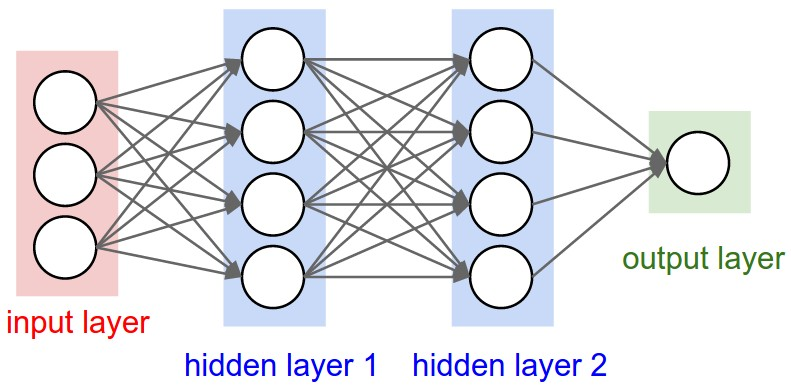
\includegraphics[scale=0.35]{mlp.jpeg}
\end{figure}
\end{frame}

	
	

\begin{frame}
\frametitle{Стохастический градиентный спуск (SGD) и его модификации}	

\begin{equation}
\theta_{t+1} = \theta_t - \eta \nabla f(\theta_t)
\end{equation}

Наиболее популярные модификации:

\begin{itemize}
\item Стохастический градиентный спуск с инерцией (SGDm) %учитываем с некоторым весом градиент на предыдущей итерации
\item Метод адаптивного градиента (Adagrad) %перемасштабируем вес каждого элемента градиента с учетом величины суммы квадратов прошлых градиентов
\item Метод адаптивного скользящего среднего градиентов (RMSprop) %то же самое, что Адаград, только поддерживается экспоненциальное скользящее среднее прошлых градиентов -- оценка второго момента градиента
\item Метод адаптивного шага обучения (Adadelta) %работает, как RMSprop, но добавлен хитрый моментум
\item Метод адаптивной инерции (Adam) %точно такой же, как RMSprop, только добавлен моментум в числитель шага
\end{itemize}

\end{frame}

\begin{frame}
\frametitle{Интуиция методов}
\begin{figure}
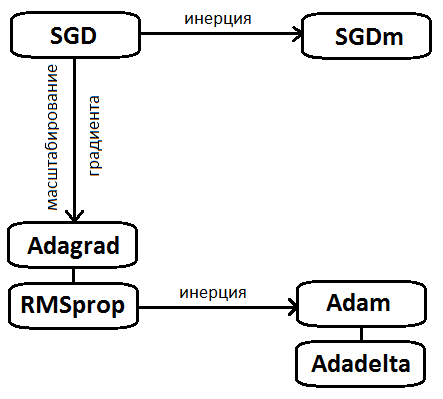
\includegraphics[scale=0.5]{methods.png}
\end{figure}
\end{frame}


\begin{frame}
	\frametitle{Ковариационный сдвиг и батч-нормализация}
	
\begin{itemize}
\item Проблема \textit{ковариационного сдвига} (Shimodaira, 2000)
\item Нормализация входных данных  (LeCun  et  al.,  1998b;  Wiesler \&  Ney,
2011)
\item Батч-нормализация (Ioffe \& Szegedy, 2015)

\begin{equation}
\hat{x}^k = \frac{x^k - \mathbb{E}[x^k]}{\sqrt{\mathrm{Var}[x^k]}}
\end{equation}


\begin{equation}
y^k = \gamma^k \hat{x}^k + \beta^k
\end{equation}
\end{itemize}

\end{frame}


\begin{frame}
	\frametitle{Батч-нормализация}

\begin{itemize}
\item Уменьшает ковариационный сдвиг и ускоряет обучение.
\item Является дифференцируемым преобразованием.
\item Использует мини-батчи, тем самым подходит для работы с большими данными.
\end{itemize}

Авторы идеи (Ioffe \& Szegedy, 2015) обучали нейронную сеть с батч-нормализацией с помощью метода SGD. Мы исследуем совместимость батч-нормализации и модификаций SGD, расмотренных выше.
\end{frame}


\section{Эксперименты}

\begin{frame} 
\frametitle{Датасеты}	
В рамках работы мы проводили экспериментальные исследования на следующих датасетах:
\begin{itemize}
\item MNIST (70 тыс. рукописных цифр --- 10 классов)
\item CIFAR-10 (60 тыс. изображений --- 10 классов)
\end{itemize}	

\begin{minipage}{0.45\linewidth}
\begin{figure}
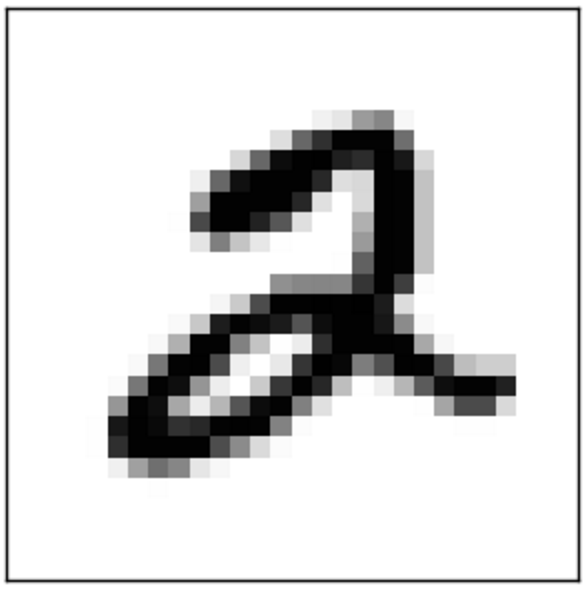
\includegraphics[scale=0.3]{mnist_img.png}
\end{figure}
\end{minipage} \hfill
\begin{minipage}{0.45\linewidth}
\begin{figure}
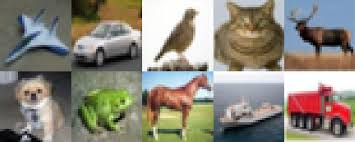
\includegraphics[scale=0.4]{cifar_img.jpeg}
\end{figure}
\end{minipage}

\end{frame}

\begin{frame}
	\frametitle{Архитектуры}
Для экспериментов использовались следующие архитектуры:
\begin{itemize}
\item полносвязная сеть (MLP): 3 полносвязных скрытых слоя по 100 нейронов;
\item сверточная сеть (CNN): 2 сверточных слоя с макс-пулингом, затем один полносвязный слой с 256 нейронами;
\item полносвязная глубокая сеть (deep MLP):  20 полносвязных скрытых слоёв по 30 нейронов;
\item сверточная глубокая сеть (deep CNN): 5 сверточных подсетей (каждая состоит из 3-х сверточных слоёв с макс-пулингом), затем один полносвязный слой с 256 нейронами.
\end{itemize}
\end{frame}


\begin{frame}
	\frametitle{Гипотезы}
	
\begin{itemize}
\item Добавление батч-нормализации в сеть увеличивает скорость сходимости обучения сети для всех методов.
\item Чем метод сложнее, тем батч-нормализация слабее ускоряет его сходимость.
\item Батч-нормализация сильнее проявляет ускорение обучения на глубоких сетях.
\end{itemize}

\end{frame}

\begin{frame}
	\frametitle{Результаты}
	
\begin{itemize}
\item Предварительно для каждого метода на различных датасетах и архитектурах был подобран оптимальный шаг обучения.
\item Для измерения повышения качества работы методов был выбран показатель относительного улучшения:
\begin{equation}
\mathrm{rel} = \frac{y - x}{100 - x},\ rel \leq 1
\end{equation}
\end{itemize}

\end{frame}

%\begin{frame}
%\begin{figure}
%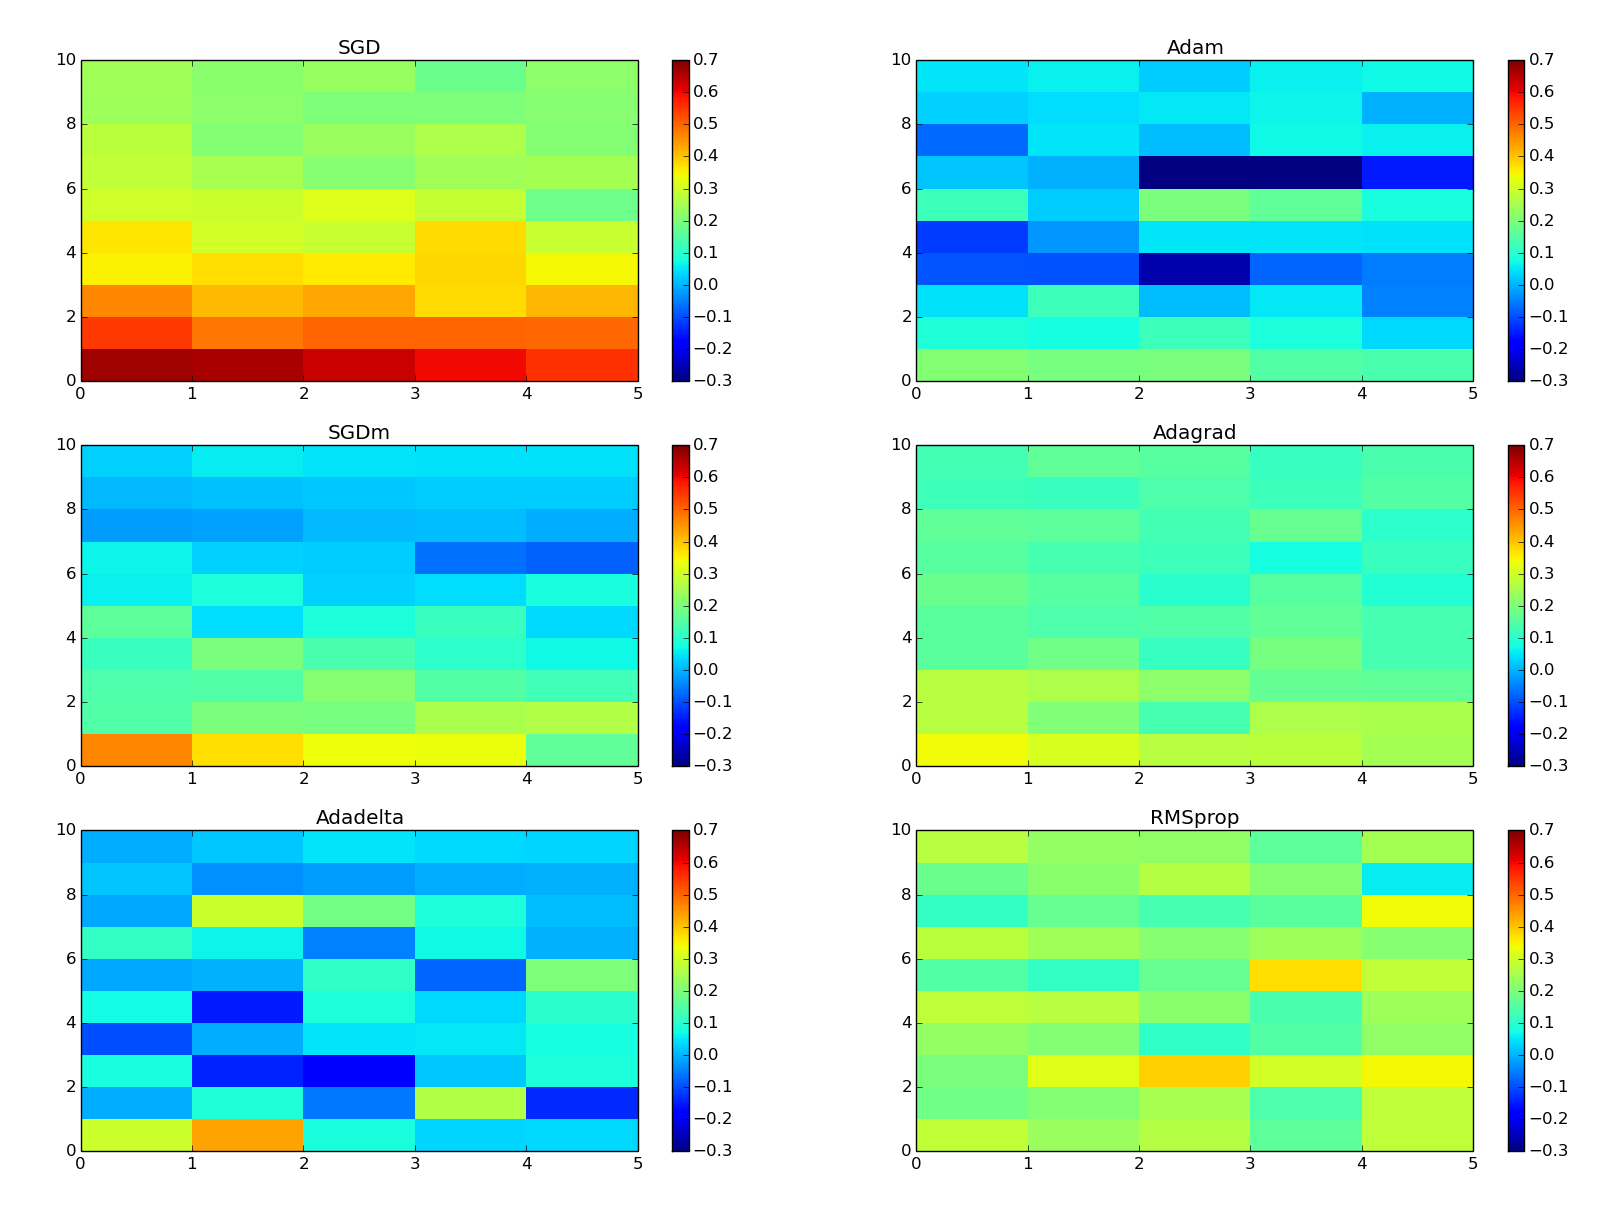
\includegraphics[scale=0.23]{map_mlp_mnist.png}
%\caption{Относительное улучшение по эпохам, MLP + MNIST}
%\end{figure}
%\end{frame}




%\begin{frame}
%	\frametitle{\small Влияние БН на все методы}
%\begin{table}[h!]
%\centering
%\scriptsize
%\begin{tabular}{|c|p{1.5cm}|p{1.5cm}|p{1.5cm}|p{1.5cm}|}\hline
%\textbf{Методы} & \textbf{MNIST +~MLP} & \textbf{CIFAR-10 +~MLP} & \textbf{MNIST +~CNN} & \textbf{CIFAR-10 +~CNN} \\\hline
%\rule{0cm}{0.3cm}
%\textbf{SGD} & \textbf{0.24} & \textbf{0.2} & \textbf{0.35} & \textbf{0.36} \\\hline
%\rule{0cm}{0.3cm}
%SGDm & 0.06 & 0.1 & 0.29 & 0.25 \\\hline
%\rule{0cm}{0.3cm}
%Adam & 0.05 & 0.09 & 0.13 & 0.14 \\\hline
%\rule{0cm}{0.3cm}
%Adagrad & 0.13 & 0.17 & 0.3 & 0.33 \\\hline
%\rule{0cm}{0.3cm}
%Adadelta & 0.03 & 0.11 & 0.19 & 0.2 \\\hline
%\rule{0cm}{0.3cm}
%RMSprop & 0.22 & 0.16 & 0.24 & 0.19 \\\hline
%\end{tabular}
%\caption{\scriptsize Улучшение качества всех методов при добавлении БН} \label{table:1}
%\end{table}
%\end{frame}


\begin{frame}
	\frametitle{\small Влияние БН на сверточные сети, топ-3 наименьшего улучшения}
\begin{table}[h!]
\centering
\begin{minipage}{1\linewidth}
\centering
\scriptsize
\begin{tabular}{|c|c|c|c|c|c|c|c|c|c|}\hline
\textbf{Номер эпохи} & \textbf{2} & \textbf{5}  & \textbf{20}  & \textbf{35} & \textbf{50} \\\hline

SGD & 0.64 & 0.57  & 0.48  & 0.49 & 0.37 \\\hline

SGDm & 0.7 & 0.52  & 0.47  & 0.34 & 0.3 \\\hline

\textbf{Adam} & \textbf{0.44} & \textbf{0.17}  & \textbf{0.29}  & \textbf{0.15} & \textbf{0.11} \\\hline

Adagrad & 0.46 & 0.38  & 0.31 & \textbf{0.3} & 0.33 \\\hline

\textbf{Adadelta} & \textbf{0.19} & \textbf{0.07}  & \textbf{0.23} & \textbf{0.15} & \textbf{0.18} \\\hline

\textbf{RMSprop} & \textbf{0.34} & \textbf{0.22}  & \textbf{0.11}  & 0.36 & \textbf{0.27} \\\hline
\end{tabular}
\caption{\scriptsize Улучшения качества по эпохам MNIST, CNN} 
\end{minipage} \vfill
\begin{minipage}{1\linewidth}
\centering
\scriptsize
\begin{tabular}{|c|c|c|c|c|c|}\hline
\textbf{Номер эпохи} & \textbf{2} & \textbf{5} & \textbf{20} & \textbf{35} & \textbf{50} \\\hline
SGD & 0.32 & 0.4 & 0.3 & 0.34 & 0.32 \\\hline

SGDm & 0.34 & 0.34 & 0.35 & 0.27 & 0.24 \\\hline

\textbf{Adam} & \textbf{0.19} & \textbf{0.22} & \textbf{0.23} &\textbf{ 0.2} & \textbf{0.15} \\\hline

Adagrad & \textbf{0.26} & \textbf{0.26} & 0.35 & 0.37 & 0.35 \\\hline

\textbf{Adadelta} & 0.27 & 0.34 & \textbf{0.17} & \textbf{0.22} & \textbf{0.22} \\\hline

\textbf{RMSprop} & \textbf{0.23} & \textbf{0.22} & \textbf{0.26} & \textbf{0.21} & \textbf{0.19} \\\hline

\end{tabular}
\caption{\scriptsize Улучшения качества по эпохам CIFAR-10, CNN}
\end{minipage}
\end{table}
\end{frame}



\begin{frame}
	\frametitle{\small Влияние БН на полносвязные сети, топ-3 наименьшего улучшения}
\begin{table}[h!]
\centering
\begin{minipage}{1\linewidth}
\centering
\scriptsize
\begin{tabular}{|c|c|c|c|c|c|}\hline
\textbf{Номер эпохи} & \textbf{2} & \textbf{5} & \textbf{10} & \textbf{25} & \textbf{50} \\\hline
SGD & 0.67 & 0.63 & 0.42 & 0.25 & 0.22 \\\hline

\textbf{SGDm} & 0.47 & 0.34 &  \textbf{0.13} &  \color{red}\textbf{-0.08} &  \textbf{0.05} \\\hline

\textbf{Adam} &  \textbf{0.21} &  \textbf{0.2} & \color{red}\textbf{-0.05} & \color{red}\textbf{-0.15} & \textbf{0.07} \\\hline

Adagrad & 0.34 & 0.27 & 0.17 & 0.12 & 0.14 \\\hline

\textbf{Adadelta} & \textbf{0.3} & \textbf{0.08} & \textbf{0.08} & \color{red}\textbf{-0.0} & \textbf{0.03} \\\hline

RMSprop & \textbf{0.28} & \textbf{0.27} & 0.35 & 0.21 & 0.25 \\\hline

\end{tabular}
\caption{\scriptsize Улучшения качества по эпохам MNIST, MLP}
\end{minipage} \vfill
\begin{minipage}{1\linewidth}
\centering
\scriptsize
\begin{tabular}{|c|c|c|c|c|c|c|}\hline
\textbf{Номер эпохи} & \textbf{2} & \textbf{5} & \textbf{10} & \textbf{25} & \textbf{50} \\\hline

SGD & 0.23 & 0.18 & 0.22 & 0.21 & 0.17 \\\hline

\textbf{SGDm} & \textbf{0.17} & \textbf{0.13} & \textbf{0.15} & \textbf{0.13} & \textbf{0.1} \\\hline

\textbf{Adam} & \textbf{0.13} &\textbf{ 0.12} & \textbf{0.11} & \textbf{0.1}3 & \textbf{0.12} \\\hline

Adagrad & 0.25 & 0.23 & 0.23 & 0.18 & 0.17 \\\hline

\textbf{Adadelta} & \textbf{0.18} & \textbf{0.14} & \textbf{0.19} & \textbf{0.17} & \textbf{0.15} \\\hline

RMSprop & 0.2 & 0.18 & 0.21 & 0.22 & 0.16 \\\hline

\end{tabular}
\caption{\scriptsize Улучшения качества по эпохам CIFAR-10, MLP}
\end{minipage}

\end{table}
\end{frame}



%\begin{frame}
%	\frametitle{\small Зависимость влияния БН от первоначального качества}
%\begin{table}
%\begin{minipage}{1\linewidth}
%\centering
%\scriptsize
%\begin{tabular}{|c|c|c|c|c|c|}\hline
%\textbf{Номер эпохи} & \textbf{1} & \textbf{2} & \textbf{25} & \textbf{35} & \textbf{50} \\\hline
%SGD & 0.32 & 0.4 & 0.3 & 0.34 & 0.32 \\\hline
%
%SGDm & 0.34 & 0.34 & 0.35 & 0.27 & 0.24 \\\hline
%
%\textbf{Adam} & \textbf{0.19} & \textbf{0.22} & \textbf{0.23} &\textbf{ 0.2} & \textbf{0.15} \\\hline
%
%Adagrad & \textbf{0.26} & \textbf{0.26} & 0.35 & 0.37 & 0.35 \\\hline
%
%\textbf{Adadelta} & 0.27 & 0.34 & \textbf{0.17} & \textbf{0.22} & \textbf{0.22} \\\hline
%
%\textbf{RMSprop} & \textbf{0.23} & \textbf{0.22} & \textbf{0.26} & \textbf{0.21} & \textbf{0.19} \\\hline
%
%\end{tabular}
%\caption{\scriptsize Улучшения качества по эпохам CIFAR-10, CNN. Жирным выделены топ-3 наименьшего улучшения}
%\end{minipage} \vfill
%\begin{minipage}{1\linewidth}
%\centering
%\scriptsize
%\begin{tabular}{|c|c|c|c|c|c|}\hline
%\textbf{Номер эпохи} & \textbf{1} & \textbf{2} & \textbf{25} & \textbf{35} & \textbf{50} \\\hline
%{SGD} & 24.26 & 22.14 & 58.95 & 63.23 & 65.45 \\\hline
%
%{SGDm} & \color{green}\textbf{30.03} & \color{green}\textbf{37.98} & \color{green}\textbf{64.37} & 68.3 & \color{green}\textbf{71.54} \\\hline 
%
%\textbf{Adam} & \color{green}\textbf{43.28} &\color{green}\textbf{47.3} & \color{green}\textbf{68.02} & \color{green}\textbf{70.79} & \color{green}\textbf{72.54} \\\hline
%
%{Adagrad} & 29.82 & 37.25 & 60.86 & 62.35 & 64.63 \\\hline
%
%\textbf{Adadelta} & \color{green}\textbf{31.31} & 32.96 & \color{green}\textbf{67.12} & \color{green}\textbf{70.56} & \color{green}\textbf{70.81} \\\hline
%
%\textbf{RMSprop} & 25.6 & \color{green}\textbf{39.89} & 64.24 & \color{green}\textbf{68.96} & 70.31 \\\hline
%
%\end{tabular}
%\caption{\scriptsize Качество методов по эпохам на CIFAR-10, CNN. Выделены топ-3 лучшего качества}
%\end{minipage} 
%\end{table}
%\end{frame}


%\begin{frame}
%	\frametitle{\small БН и глубокая полносвязная сеть}
%\begin{table}[h!]
%\begin{minipage}{1\linewidth}
%\centering
%\scriptsize
%\begin{tabular}{|c|c|c|c|c|c|}\hline
%\textbf{Номер эпохи} & \textbf{2} & \textbf{5} & \textbf{10} & \textbf{25} & \textbf{50} \\\hline
%
%SGD & 0.84 & 0.9 & 0.94 & 0.93 & 0.7 \\\hline
%
%SGDm & 0.8 & 0.83 & 0.32 & 0.19 & 0.03 \\\hline
%
%Adam & 0.72 & 0.66 & 0.58 & 0.4 & 0.28 \\\hline
%
%Adagrad & 0.85 & 0.84 & 0.45 & 0.37 & 0.37 \\\hline
%
%Adadelta & 0.58 & 0.69 & 0.27 & 0.18 & 0.14 \\\hline
%
%RMSprop & 0.72 & 0.82 & 0.45 & 0.39 & 0.37 \\\hline
%\end{tabular}
%\end{minipage} \vfill
%\caption{\scriptsize Улучшения качества для MNIST, deep MLP}
%\begin{minipage}{1\linewidth}
%\centering
%\scriptsize
%\begin{tabular}{|c|c|c|c|c|c|}\hline
%\textbf{Номер эпохи} & \textbf{2} & \textbf{5} & \textbf{10} & \textbf{25} & \textbf{50} \\\hline
%SGD & 0.67 & 0.63 & 0.42 & 0.25 & 0.22 \\\hline
%
%{SGDm} & 0.47 & 0.34 &  {0.13} &  {-0.08} &  {0.05} \\\hline
%
%{Adam} &  {0.21} &  {0.2} & {-0.05} & {-0.15} & {0.07} \\\hline
%
%Adagrad & 0.34 & 0.27 & 0.17 & 0.12 & 0.14 \\\hline
%
%{Adadelta} & {0.3} & {0.08} & {0.08} & {-0.0} & {0.03} \\\hline
%
%RMSprop & {0.28} & {0.27} & 0.35 & 0.21 & 0.25 \\\hline
%
%\end{tabular}
%\end{minipage}
%\caption{\scriptsize Улучшения качества для MNIST, MLP}
%\end{table}
%\end{frame}



\begin{frame}
	\frametitle{\small БН и глубокая сверточная сеть}
\begin{table}[h!]

\centering
\scriptsize
\begin{tabular}{|c|c|c|c|c|c|}\hline
\textbf{Номер эпохи} & \textbf{2} & \textbf{5} & \textbf{20} & \textbf{35} & \textbf{50} \\\hline
SGD & \color{green}{0.1} & \color{green}{0.23} & \color{green}{0.41} & \color{green}{0.44} & \color{green}{0.34} \\\hline

SGDm & \color{green}{0.1} & \color{green}{0.31} & \color{green}{0.36} & \color{green}{0.42} & \color{green}{0.18} \\\hline

Adam & \color{green}{0.17} & \color{green}{0.35} & \color{green}{0.37} & \color{green}{0.41} & \color{green}{0.37} \\\hline

Adagrad & \color{red}{-0.05} & \color{green}{0.21} & \color{green}{0.24} & \color{green}{0.28} & \color{green}{0.28} \\\hline

Adadelta & \color{green}{0.14} & \color{green}{0.25} & \color{green}{0.51} & \color{green}{0.45} & \color{green}{0.43} \\\hline

RMSprop & \color{red}{-0.1} & \color{green}{0.27} & \color{green}{0.37} & \color{green}{0.46} & \color{green}{0.42} \\\hline

\end{tabular}
\caption{\scriptsize Разница в улучшении качества deep CNN и CNN для CIFAR-10}
\end{table}
\end{frame}

\begin{frame}
	\frametitle{\small Комбинация БН с методом Adam}
\begin{figure}
\centering
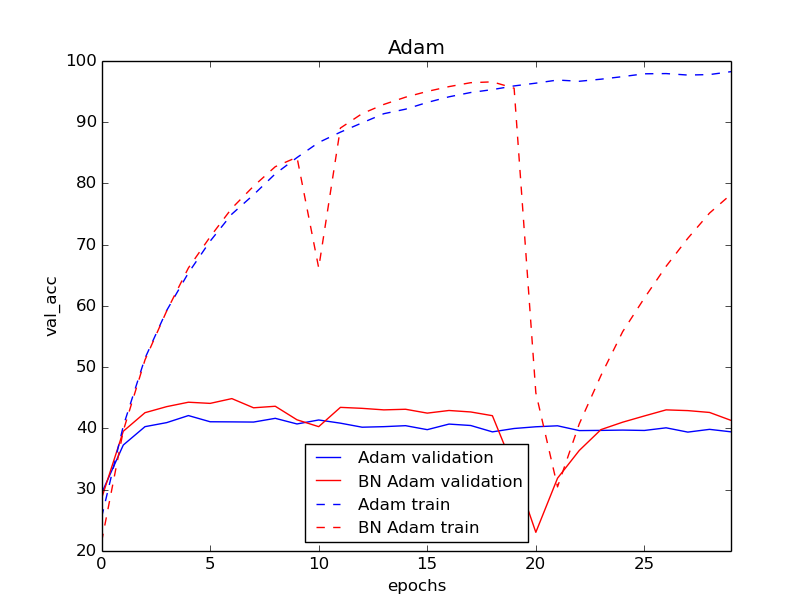
\includegraphics[scale=0.4]{adam_shallow.png}
\end{figure}
\end{frame}


\section{Выводы}

%\begin{frame}
%	\frametitle{Выводы}
%\begin{itemize}
%\item Добавление батч-нормализации в сеть, в основном, улучшает качество методов.
%\item На сверточных сетях слабее улучшаются методы Adam, Adadelta и RMSprop, на полносвязных --- SGDm, Adam и Adadelta.
%\item Чем метод сложнее, тем батч-нормализация слабее ускоряет его сходимость.
%\item Батч-нормализации сильнее проявляет ускорение обучения на глубоких сетях.
%\end{itemize}
%\end{frame}


\begin{frame}
	\frametitle{Рекомендации}
\begin{itemize}
\item Для полносвязной неглубокой архитектуры сети батч-нормализацию стоит применять к более простым методам.
\item Для глубоких сетей важно использовать батч-нормализацию.
\item Если время или количество эпох ограничено и очень мало, то однозначно стоит добавить в сеть батч-нормализацию.
\item Для метода Adam с батч-нормализацией нужно быть аккуратным: чтобы не возникло проблем при обучении, требуется аккуратно подобрать параметры метода.
\end{itemize}
\end{frame}



%\begin{frame}
%\frametitle{На защиту выносится:}
%\begin{enumerate}
%\item Экспериментальные исследования модификаций стохастического градиентного спуска для обучения нейронных сетей с и без батч-нормализации.
%\item Подтверждение гипотезы об ускорении сходимости модификаций метода стохастического градиентного спуска при добавлении в сеть батч-нормализации.
%\item Подтверждение гипотезы о зависимости величины улучшения качества работы метода при добавлении в сеть батч-нормализации от сложности метода.
%\end{enumerate}
%\end{frame}

\begin{frame}
\frametitle{На защиту выносится:}
\begin{enumerate}
\item Экспериментальное исследование гипотезы о зависимости величины улучшения качества работы метода при добавлении в сеть батч-нормализации от сложности метода.
\item Экспериментальное исследование влияния глубины нейронной сети на совместимость батч-нормализации и модификаций метода стохастического градиентного спуска.
\item Рекомендации по применению батч-нормализации для рассмотренных архитектур и методов.
\end{enumerate}
\end{frame}



\begin{frame}
\frametitle{SGD}
\[\theta_{t+1} = \theta_t - \eta \nabla F(\theta)\]	
\end{frame}

\begin{frame}
\frametitle{SGD momentum}
\[v_{t+1} = \mu v_t - \eta \nabla F(\theta)\]
\[\theta_{t+1} = \theta_t + v_{t+1}\]	
\end{frame}

\begin{frame}
\frametitle{Adagrad}
\[g_{t+1} = g_t + \nabla F(\theta) ^2\]
\[\theta_{t+1} = \theta_t - \frac{\eta \nabla F(\theta)}{\sqrt{g_{t+1}} + \epsilon}\]	
\end{frame}

\begin{frame}
\frametitle{RMSprop}
\[g_{t+1} = \gamma g_t + (1 - \gamma) \nabla F(\theta)^2\]
\[\theta_{t+1} = \theta_t - \frac{\eta \nabla F(\theta)}{\sqrt{g_{t+1} + \epsilon}}\]	
\end{frame}

\begin{frame}
\frametitle{Adadelta}
\[g_{t+1} = \gamma g_t + (1 - \gamma) \nabla F(\theta)^2\]
\[v_{t+1} = - \frac{\sqrt{x_t + \epsilon} \nabla F(\theta)}{\sqrt{g_{t+1} + \epsilon}}\]
\[x_{t+1} = \gamma x_t + (1 - \gamma) v_{t+1}^2\]
\[\theta_{t+1} = \theta_t + v_{t+1}\]	
\end{frame}

\begin{frame}
\frametitle{Adam}
\[m_{t+1} = \gamma_1 m_t + (1 - \gamma_1) \nabla F(\theta)\]
\[g_{t+1} = \gamma_2 g_t + (1 - \gamma_2) \nabla F(\theta)^2\]
\[\hat{m}_{t+1} = \frac{m_{t+1}}{1 - \gamma_1^{t+1}}\]
\[\hat{g}_{t+1} = \frac{m_{t+1}}{1 - \gamma_2^{t+1}}\]
\[\theta_{t+1} = \theta_t - \frac{\eta \hat{m}_{t+1}}{\sqrt{\hat{g}_{t+1}} + \epsilon}\]	
\end{frame}

	
\end{document}
